% !TeX spellcheck = en_US

% Kompatibilität zu Libs
% DBs zu hohe Latenz
% Der Plan = GIS Layer
\chapter{Software Design}
\label{sec:software_design}
This chapter discusses the current state and possible solutions for working with GIS inside the LIFE simulation system.



\section{Current state}
Currently the GIS support inside MARS is partial, some components of the environment are capable of handling GIS, while others are not supporting it yet.


\subsection{WebUI}
The WebUI does not support GIS yet. 


\subsection{Back-end Services}
The back-end services fully support GIS. The file service accepts the uploaded files and hands control over to the GIS Data Service (GDS). 

\subsubsection{GIS Data Service}
The GDS is capable of handling the most common GIS types, these are GeoTIFF, GeoJSON and Esri ASCII Grid for raster and Shapefile for vector files. The files may be provided compressed inside a .zip file or as plain files.\\
During the import the GDS determines the type of data automatically by checking the file extension. Once detected, the file is validated and the spatial reference is determined. In case of a valid geo-referenced input, the file is imported into the GeoServer for persistence.

\subsubsection{GeoServer}
The GeoServer (see section \ref{sec:GS}) and it's API are build for working with whole files. The MARS use-case requires a large amount of parallel reads, reaching from thousands to millions in a short amount of time. The GeoServer does not satisfy this demands. The retrieval of single values is not supported, since the general use-case is to work with complete files and the performance for retrieving data is very poor which will require a better solution.\\
figure \ref{img:gs-read-performance} shows that the response time for various data types and storage solutions is always above 2 seconds. \cite{Pandey2016} argues that disk-based systems are generally not fast enough for real-time analysis.

\begin{figure}[H]
	\centering
	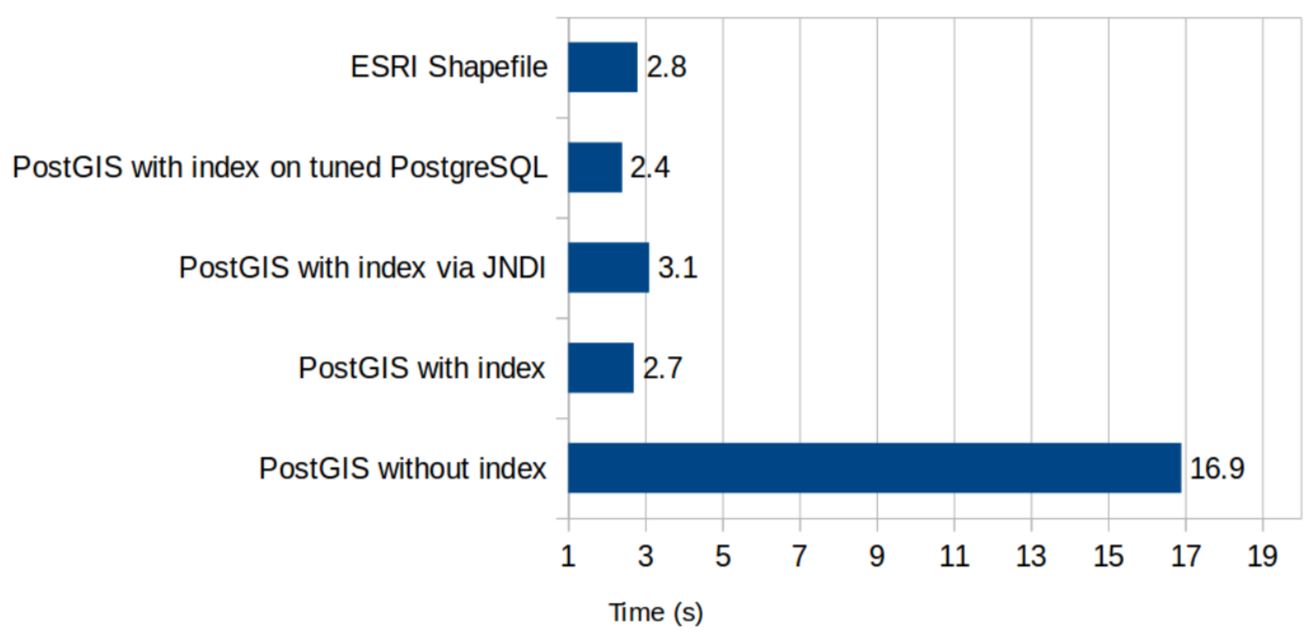
\includegraphics[width=0.8\columnwidth]{res/gs-read-performance}\\
	\caption[]{GeoServer average time of response by \cite{ruuvzivcka2016comparing}}
	\label{img:gs-read-performance}
\end{figure}



\section{Methods of Resolutions}
This section discusses the possible solutions for the given problem and rules out some less fitting approaches bases on performance metrics.\\
As mentioned before, reading data from the GeoServer during the simulation does not seam feasible inside a high performance environment. However, it was still tested to serve as a reference point for other possible solutions.\\
Hadoop-GIS with MapReduce as suggested by \cite{Wang2011} offers very good scalability but does not support the high IO and low latency focused use-case of the MARS system. GeoMesa and Vector Cluster as suggested by \cite{Toups2016} was not taken into closer consideration, since PostGIS offered a better performance. Vertica as proposed by \cite{Pavlo2009} were ruled out due to lack of performance as well.\\
Databases are a common, fast and flexible way to safely store data and it therefore seem ideal to use in the current scenario. But given the extreme performance requirements, it might be beneficial to use alternative approaches. Figure \ref{img:spatial-queries} shows that local GIS libraries tend to drastically outperform database solutions. For this reason they were also considered during the evaluation.\\

\begin{figure}[H]
	\centering
	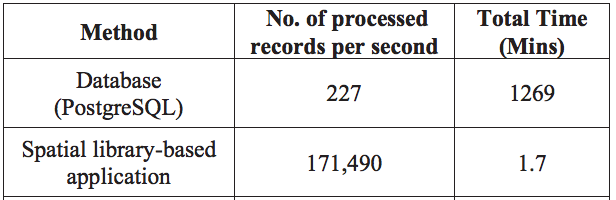
\includegraphics[width=0.6\columnwidth]{res/spatial-queries}\\
	\caption[]{Processing time on spatial queries by \cite{Witayangkurn2012}}
	\label{img:spatial-queries}
\end{figure}

There are two major databases with GIS support, PostGIS and MongoDB. Both offer competitive vector GIS performance, as figure \ref{img:mongo-vs-postgres} shows. Thus they were both tested as possible solutions.

\begin{figure}[H]
	\centering
	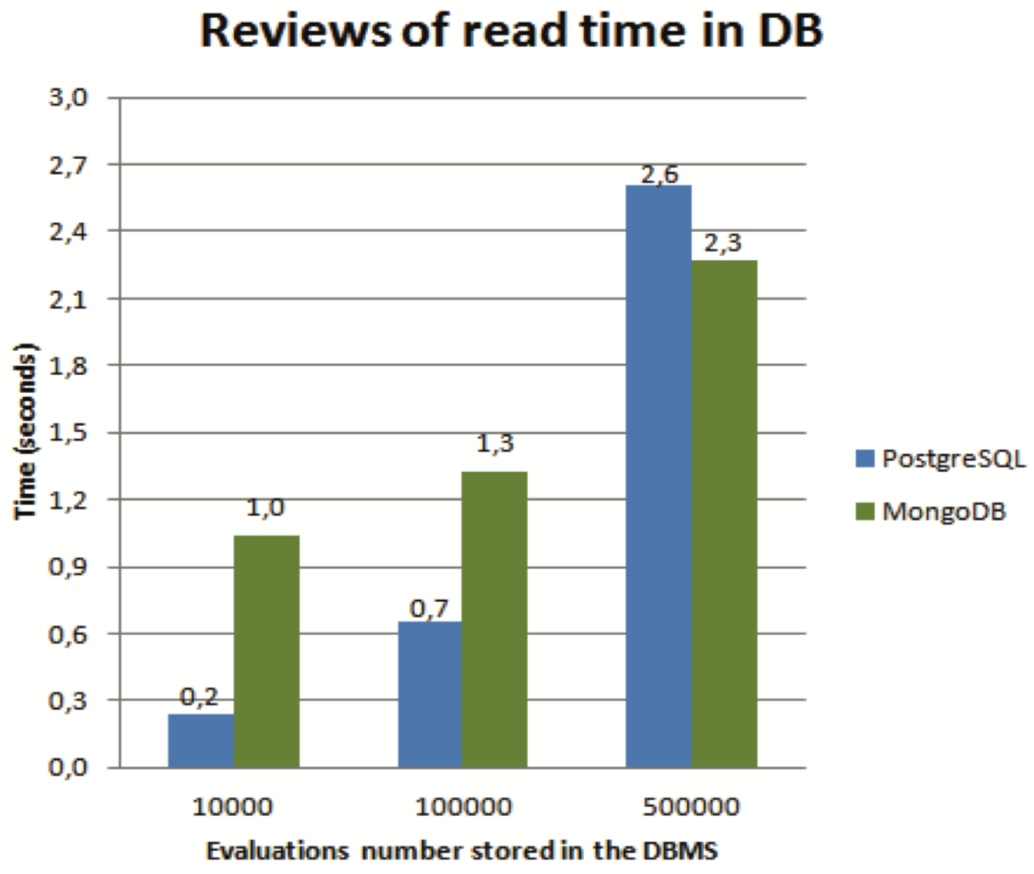
\includegraphics[width=0.6\columnwidth]{res/mongo-vs-postgres}\\
	\caption[]{Comparison of the times of the read of the evaluation data in the Database PostgreSQL and MongoDB by \cite{Maia2016}}
	\label{img:mongo-vs-postgres}
\end{figure}


\subsection{Performance Tests}
The previously mentioned techniques suggest that the use of local libraries offers the best performance, due to the lack of network latency. To validate this assumption all mentioned technologies were performance tested with the same input files. A small, medium and a large size vector and raster file. The sizes were 10 KB, 6.5 MB and 105 MB. Each test performs 1,000 parallel reads and the result is the average of three separate runs. The test hardware was a Apple MacBook Pro (2016) with SSD storage, 16GB RAM and a 4x 2,7GHZ processor.\\
The results are listed in figure \ref{fig:vector_performace} for vector and \ref{fig:raster_performace} for raster inputs. Detailed analysis of the tests can be found in the following section.

\begin{figure}[H]
	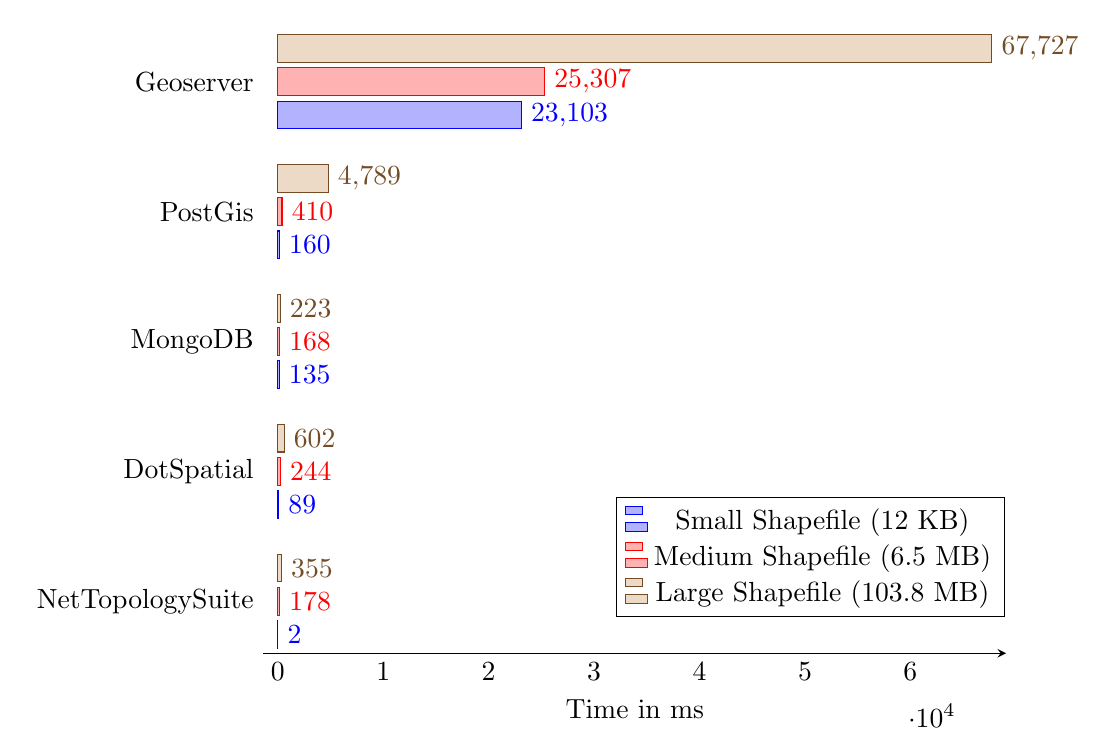
\begin{tikzpicture}
	\begin{axis}[
	xbar,
	y axis line style = { opacity = 0 },
	axis x line       = bottom,
	tickwidth         = 0pt,
	%	enlarge y limits  = 0.02,
	enlarge x limits  = 0.02,
	symbolic y coords = {NetTopologySuite, DotSpatial, MongoDB, PostGis, Geoserver},
	nodes near coords,
	height=9.5cm,
	legend style={at={(0.737,0.25)},anchor=north},
	xlabel={Time in ms},
	]
	% Small Shapefile
	\addplot coordinates {
		(23103,Geoserver)
		(160,PostGis)
		(135,MongoDB)
		(89,DotSpatial)
		(2,NetTopologySuite)
	};
	% Mid Shapefile
	\addplot coordinates {
		(25307,Geoserver)
		(410,PostGis)
		(168,MongoDB)
		(244,DotSpatial)
		(178,NetTopologySuite)
	};
	% Large Shapefile
	\addplot coordinates {
		(67727,Geoserver)
		(4789,PostGis)
		(223,MongoDB)
		(602,DotSpatial)
		(355,NetTopologySuite)
	};
	\legend{Small Shapefile (12 KB),Medium Shapefile (6.5 MB),Large Shapefile (103.8 MB)}
	\end{axis}
	\end{tikzpicture}
	\caption{Vector performance for 1k reads}
	\label{fig:vector_performace}
\end{figure}


\begin{figure}[H]
	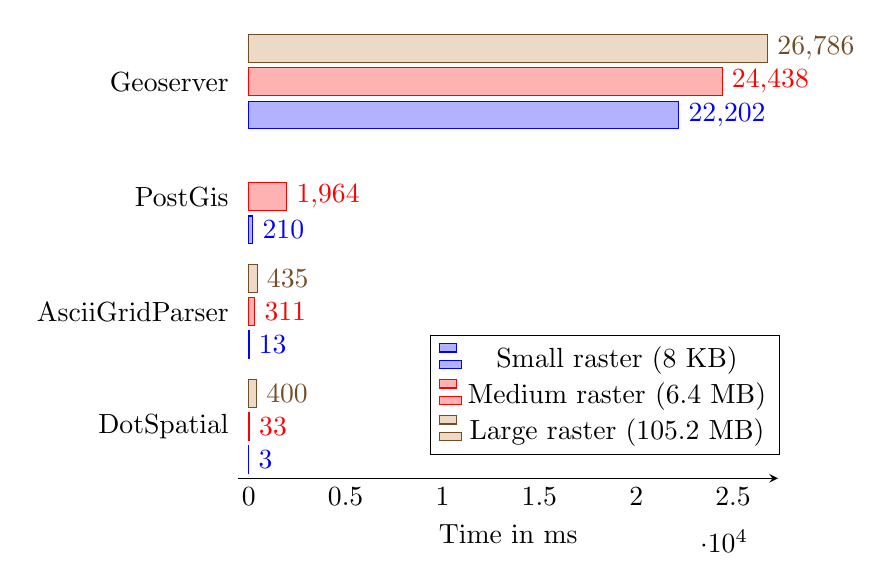
\begin{tikzpicture}
	\begin{axis}[
	xbar,
	y axis line style = { opacity = 0 },
	axis x line       = bottom,
	tickwidth         = 0pt,
	enlarge y limits  = 0.15,
	enlarge x limits  = 0.02,
	symbolic y coords = {DotSpatial, AsciiGridParser, PostGis, Geoserver},
	nodes near coords,
	legend style={at={(0.68,0.32)},anchor=north},
	xlabel={Time in ms},
	]
	% Small Rasterfile
	\addplot coordinates {
		(22202,Geoserver)
		(210,PostGis)
		(13,AsciiGridParser)
		(3,DotSpatial)
	};
	% Mid Rasterfile
	\addplot coordinates {
		(24438,Geoserver)
		(1964,PostGis)
		(311,AsciiGridParser)
		(33,DotSpatial)
	};
	% Large Rasterfile
	\addplot coordinates {
		(26786,Geoserver)
		(nan,PostGis) % 342197
		(435,AsciiGridParser)
		(400,DotSpatial)
	};
	\legend{Small raster (8 KB),Medium raster (6.4 MB),Large raster (105.2 MB)}
	\end{axis}
	\end{tikzpicture}
	\caption{Raster performance for 1k reads}
	\label{fig:raster_performace}
\end{figure}

\subsubsection{GeoServer}
As expected, the GeoServer was outperformed by all other technologies. With the best results around 22 seconds, it is clearly not suited for the task.

\subsubsection{PostGIS}
The PostGIS performance is way better than the of the GeoServer, however it did not handle the large file very well. The reading of the large vector file took over 10 times longer than the smaller file, which is surprising since the data is broken into tables. A larger table should not effect the response time by that extend.\\
The big raster file was even worse. The test crashed with an OutOfMemory exception. Limiting the parallelism of threads to 7 prevented the crash, but the results of around ~340,000 ms (5 min. 40 sec.) were not acceptable. For readability reasons, the high number was omitted from the graph.

\subsubsection{MongoDB}
MongoDB offers good overall performance for vector data. The file size does not effect the overall performance by a large extend. For the medium and large file it was even faster than the local library NetTopologySuite (NTS). Raster GIS is not supported and therefore has no test data.

\subsubsection{DotSpatial}
DotSpatial offers average vector read performance. MongoDB and NTS perform slightly better. As of August 25th 2017 the library has not been ported to .NET Core. This is why a .NET Core compatible ESRI AsciiGridParser was created.

\subsubsection{NetTopologySuite}
NTS has the best vector read performance. It does not support raster GIS. As of August 2017 NTS is available for .NET Core. The implementation of the Shapefile compatibility is currently missing, but expected to return soon (see \url{https://github.com/NetTopologySuite/NetTopologySuite/issues/184}). Therefore the GeoJSON reader was used as alternative.

\subsubsection{AsciiGridParser}
Due to the text-based nature of the format the read performance is not as good as the DotSpatial reader. It is however within the same range and offers good performance.


\subsection{Performance at Scale}
The performance at scale for the local libraries (NTS, DotSpatial and the AsciiGridParser) is different than the database solutions. The libraries open a file into RAM and read from it. The opening takes majority of the time, while reads from RAM are much faster. Since the initial opening has to be done only once, the time increase for additional reads is very low, making these solution preferable at scale.\\
The additional performance tests in \ref{fig:vector_performace_best} and \ref{fig:raster_performace_best} with 10k reads verify this. The read times for local libraries is increased by a few milliseconds, while MongoDB and PostGIS take almost 10 times as much time. With agent counts in the millions, the described effect becomes even more extreme, in favor of NTS, DotSpatial and the AsciiGridParser.


\begin{figure}[H]
	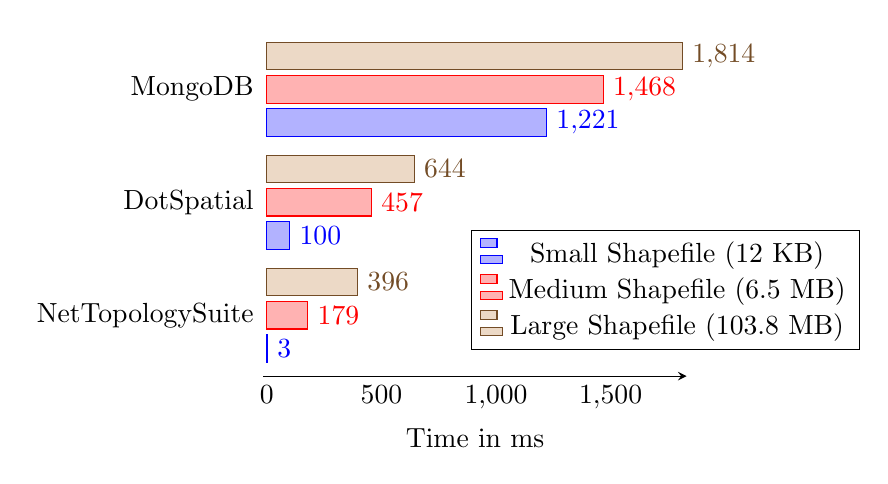
\begin{tikzpicture}
	\begin{axis}[
	xbar,
	y axis line style = { opacity = 0 },
	axis x line       = bottom,
	tickwidth         = 0pt,
	enlarge y limits  = 0.27,
	enlarge x limits  = 0.01,
	symbolic y coords = {NetTopologySuite, DotSpatial, MongoDB},
	ytick=data,
	nodes near coords,
	height=6cm,
	legend style={at={(0.95,0.42)},anchor=north},
	xlabel={Time in ms},
	]
	% Small Shapefile
	\addplot coordinates {
		(1221,MongoDB)
		(100,DotSpatial)
		(3,NetTopologySuite)
	};
	% Mid Shapefile
	\addplot coordinates {
		(1468,MongoDB)
		(457,DotSpatial)
		(179,NetTopologySuite)
	};
	% Large Shapefile
	\addplot coordinates {
		(1814,MongoDB)
		(644,DotSpatial)
		(396,NetTopologySuite)
	};
	\legend{Small Shapefile (12 KB),Medium Shapefile (6.5 MB),Large Shapefile (103.8 MB)}
	\end{axis}
	\end{tikzpicture}
	\caption{Vector performance for 10k reads}
	\label{fig:vector_performace_best}
\end{figure}

\begin{figure}[H]
	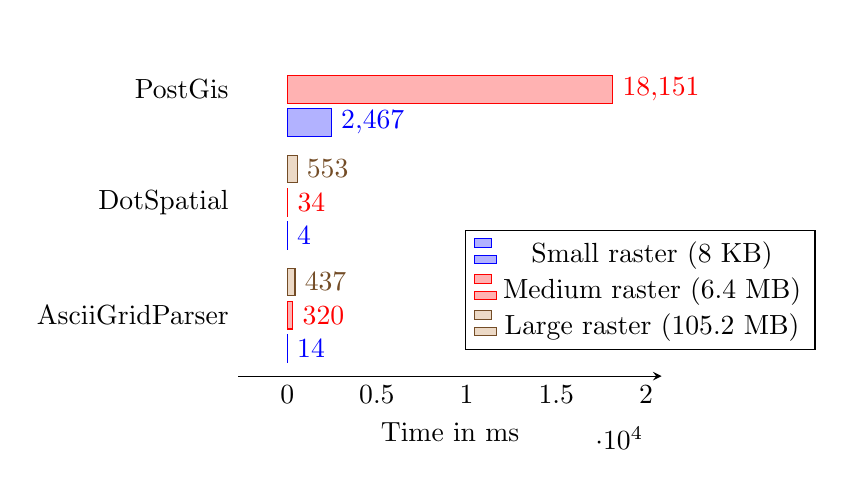
\begin{tikzpicture}
	\begin{axis}[
	xbar,
	y axis line style = { opacity = 0 },
	axis x line       = bottom,
	tickwidth         = 0pt,
	enlarge y limits  = 0.27,
	enlarge x limits  = 0.15,
	symbolic y coords = {AsciiGridParser, DotSpatial, PostGis},
	ytick=data,
	nodes near coords,
	height=6cm,
	legend style={at={(0.95,0.42)},anchor=north},
	xlabel={Time in ms},
	]
	% Small Raster
	\addplot coordinates {
		(2467,PostGis)
		(4,DotSpatial)
		(14,AsciiGridParser)
	};
	% Mid Raster
	\addplot coordinates {
		(18151,PostGis)
		(34,DotSpatial)
		(320,AsciiGridParser)
	};
	% Large Raster
	\addplot coordinates {
		(nan,PostGis)
		(553,DotSpatial)
		(437,AsciiGridParser)
	};
	\legend{Small raster (8 KB),Medium raster (6.4 MB),Large raster (105.2 MB)}
	\end{axis}
	\end{tikzpicture}
	\caption{Raster performance for 10k reads}
	\label{fig:raster_performace_best}
\end{figure}


% Describe workflow from GS to Layer
\section{Final Design}
As a result of the performance tests for compatible technologies and the requirements from section \ref{sec:requirements} the following decisions were made.


\subsection{Storage}
The files are imported using the WebUI and persisted into the GeoServer. Although the GeoServer is not fast enough for real-time analysis, as for this work needed, it is sufficient for storing the GIS files. Besides persisting data, it converts the input data into the right format for the GIS layer to use. Vector files are currently converted to GeoJSON and vector files to ESRI Shapefiles.


\subsection{GIS Layers}
Based on the requirements and technical circumstances the integration into the LIFE simulation system will be as separate layers. One for raster and one for vector data. The layers allow to initialize the inputs prior to the simulation and access them during the actual run.

\subsubsection{Vector Data}
For the vector data manipulation, NetTopologySuite will be used. It had the best performance metrics in both tests performed. It's functionality is sufficient and the project is in active development.

\subsubsection{Raster Data}
The raster data will be manipulated using the AsciiGridParser. It reads in the raster values into an multi-dimensional array. The specified mathematical functions from the requirements are implemented manually.
